\section{Introduction}
\label{sec:introduction}

Deep neural networks learn rich representations from static, independent, and identically distributed data, but a vulnerability appears as soon as training becomes sequential: the network overwrites previously acquired knowledge to accommodate new data. This phenomenon, catastrophic forgetting \cite{mccloskey:catastrophic, ratclif1990catastrophicforgetting}, is a central obstacle in machine learning: retraining from scratch on all data whenever the distribution shifts is the obvious remedy, but it is too expensive for systems that must adapt continually. Continual learning (CL) studies how to learn from a sequence of tasks without that cost, and its core difficulty is the stability--plasticity dilemma: the model must stay plastic enough to learn new distributions while staying stable enough to preserve old ones \cite{Mermillod2013Stability-Plasticity}.

Several families of techniques address forgetting, including replay, parameter and functional regularisation, optimisation-based methods, and template-based classification \cite{van_de_Ven_2025}. These methods reduce long-term forgetting, but they have historically been evaluated only at task boundaries or at coarse intervals, which hides what happens within a task. Evaluating the network continuously exposes a failure these protocols miss. \citet{delange2023continualevaluationlifelonglearning} did exactly this and identified the \textit{Stability Gap}, a transient but severe collapse in past-task accuracy that occurs immediately upon the introduction of a new task. Even a well-tuned Experience Replay model that finishes a task with high accuracy on earlier tasks passes through a deep minimum during the first hundred steps of the new task.

This matters for three reasons. First, deployed continual-learning systems are queried throughout training, so a model mid-transition commits errors its final checkpoint never would. Second, the transience is a scientific puzzle: the model clearly retains the knowledge needed to recover, so some mechanism must temporarily disrupt and then restore it. Third, relearning what was already known wastes compute, and understanding that mechanism is a prerequisite for fixing the gap efficiently.

The discovery of the gap raised an immediate question: could it be removed by better approximating the joint loss over all tasks? \citet{hess2024complementaryperspectivescontinuallearning} showed that the gap persists even under incremental joint training, where the model has access to all data from all tasks at every step. A perfect objective still produces transient forgetting, so the problem lies not in \emph{what} is optimised but in \emph{how} the optimisation proceeds.

To see why the trajectory itself produces the gap, consider the geometry of sequential optimisation. Figure~\ref{fig:loss_landscape_visualization} visualises a transition from a learned task (Task A) to a new task (Task B), a conceptual two-dimensional reduction of a high-dimensional surface that nonetheless captures the dynamics at play. The network starts at the converged minimum $A$ of Task A and must reach the joint minimum $A\cap B$. Running stochastic gradient descent (SGD) on the joint loss from $A$ follows the green curve: pulled by the steepest gradients of the joint landscape, the trajectory bows outward, leaving Task A's basin and crossing a region of higher Task-A error before converging at $A\cap B$. The dip on Task A along this arc is the stability gap.

\begin{figure*}[htbp]
    \centering
    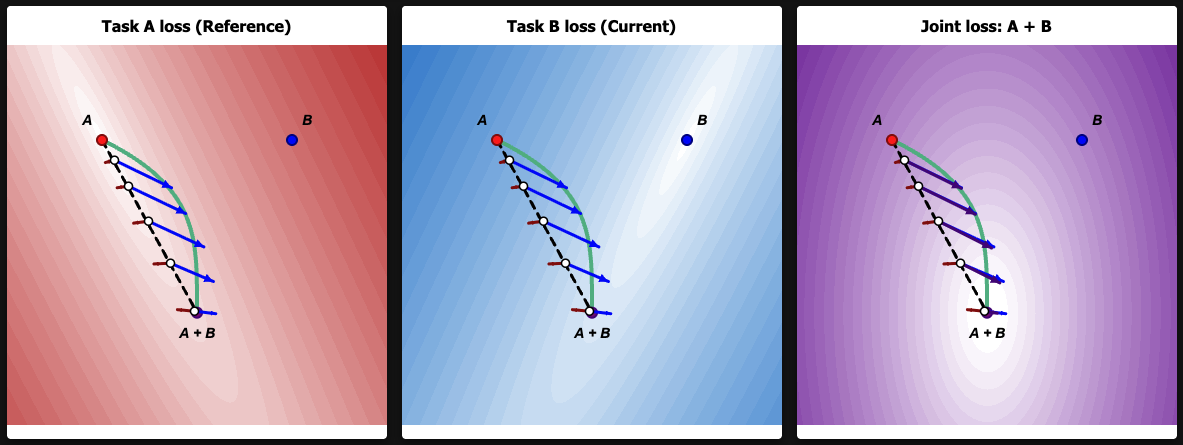
\includegraphics[width=\textwidth]{img/loss_landscape_visualization.png}
    \caption{Conceptual visualisation of the optimisation landscape at a task transition, shown over a shared two-dimensional parameter space. \textbf{Task A} (red) and \textbf{Task B} (blue) are the single-task losses with minima at $A$ and $B$; the \textbf{joint loss} $A+B$ (purple) has its minimum at $A\cap B$. The dashed line is the straight interpolation from $A$ to $A\cap B$; the green curve is the steepest-descent trajectory of the joint loss, which bows away from Task A's basin and induces the stability gap. The fourth panel shows the \textbf{$\lambda$-curriculum} loss $A+\lambda B$: a small weight $\lambda$ on Task B reshapes the basin into a valley that runs continuously from $A$ toward the joint minimum, so the optimum moves along the corridor instead of teleporting across it. Arrows are normalised to a fixed length and show gradient direction only.}
    \label{fig:loss_landscape_visualization}
\end{figure*}

This trajectory is the consequence of a discontinuity at the task boundary. While Task A is learned the optimiser descends the replay loss alone, the red basin in Figure~\ref{fig:loss_landscape_visualization}. The moment Task B begins, the objective switches in a single step to the sum of the replay and current-task losses, the purple joint basin. Its minimum at $A\cap B$ replaces the red one from one step to the next. The parameters do not move during this switch, yet the minimum they are chasing jumps from $\theta_A^*$ to $\theta_{\text{joint}}^*$. We call this \emph{landscape teleportation}: from the optimiser's point of view the surface it was descending disappears and is replaced by another whose minimum lies elsewhere.

The teleportation does more than redirect the optimiser along a curved path; it also makes the very first step after the switch lopsided. At $\theta_A^*$ the replay gradient is near zero, because the optimiser has converged on Task A, while the current-task gradient is large, because Task B is still unlearned. The summed update is therefore dominated by the new-task gradient, and SGD takes a long step out of Task A's basin before the still-negligible replay term can pull it back. This magnitude imbalance compounds the trajectory effect: not only does the descent path bow away from Task A's minimum, the first step along it is the largest and the least opposed, which is why the dip is steepest in the first updates after a task switch \citep{delange2023continualevaluationlifelonglearning}. A finite replay buffer adds a third, smaller error: it estimates the past-task gradient from a handful of stored samples rather than from all past data, so even the replay signal it supplies is noisy. Trajectory effect, magnitude asymmetry, and estimator variance are the three contributors to the gap; Section~\ref{sec:account} makes their decomposition precise and the experiments measure each in isolation.

Existing methods take this discontinuity as given. They accept that the objective jumps at the task boundary and instead make the optimiser robust to the jump, constraining each SGD update with information about the past tasks, their gradients or local curvature, so that SGD avoids directions in which the replay loss rises sharply \cite{lopezpaz2022gradientepisodicmemorycontinual, chaudhry2019efficientlifelonglearningagem, Kirkpatrick_2017, kao2021naturalcontinuallearningsuccess}. We group these approaches under the term \emph{path-finding}: effective as they are, they navigate the broken landscape without removing the break.

This thesis takes the opposite route. Rather than steer the optimiser carefully across a discontinuity, we propose removing the discontinuity itself, an approach we call \emph{landscape-shaping}. We instantiate it as the \textbf{$\lambda$-curriculum}: instead of switching the objective from the replay loss to the joint loss in a single step, the curriculum ramps the current-task loss weight from $0$ to $1$ over the first $N$ steps of each transition,
\begin{equation}
    \begin{aligned}
        L_\lambda(t) & = L_{\text{replay}} + \lambda(t)\, L_{\text{current}}, \\
        \lambda(t)   & = \mathrm{clip}\!\left(\tfrac{t}{N}, 0, 1\right),
    \end{aligned}
    \label{eq:lambda_curriculum}
\end{equation}
so the optimum $\Theta^*(\lambda)$ traces a continuous curve from $\theta_A^*$ (at $\lambda=0$) to $\theta_{\text{joint}}^*$ (at $\lambda=1$), and the model follows this moving valley instead of being teleported across the discontinuity (fourth panel of Figure~\ref{fig:loss_landscape_visualization}). That such a continuous low-loss route from $\theta_A^*$ to $\theta_{\text{joint}}^*$ exists at all is what work on linear mode connectivity \citep{draxler2019essentiallybarriersneuralnetwork, garipov2018losssurfacesmodeconnectivity} establishes: distinct optima are often joined by simple paths of near-constant loss --- the dashed corridor in Figure~\ref{fig:loss_landscape_visualization} --- and the curriculum's role is to keep the optimiser on that route rather than let it bow away. Because the optimum now moves continuously, the curriculum addresses two of the three contributors at once. It removes the trajectory effect, since the descent no longer bows away from Task A's basin (the green curve), and it tempers the magnitude imbalance, since the large new-task gradient is introduced gradually rather than dominating the first step. Only the third contributor, the variance of the finite-buffer estimator, is independent of the schedule and left untouched. Treating the task-boundary discontinuity as the object to be fixed is the central contribution of this thesis; Section~\ref{sec:theory} makes the argument precise.

Two refinements extend the basic curriculum. The linear ramp requires choosing the length $N$; an \textbf{adaptive schedule} removes this knob by setting $\lambda(t)$ from the live ratio of replay to current-task gradient magnitudes. Because that ratio can hold $\lambda$ near zero for the first steps and stall progress on the new task, a \textbf{$\lambda_{\min}$ floor} keeps the current-task gradient present from step one without re-introducing the depth the curriculum removes. Independently, \textbf{momentum} acts as a low-pass filter on the per-step accuracy oscillation that the continuous-limit argument abstracts away, suppressing mini-batch noise while preserving the slow drift along $\Theta^*(\lambda)$.

The remainder of this thesis develops these ideas. Section~\ref{sec:literature} reviews continual learning, Experience Replay, the path-finding methods we compare against, the stability-gap literature, and two lines of work --- blurry task boundaries and mode connectivity --- that bear on the curriculum. Section~\ref{sec:account} then sets out the thesis's own account of the gap: it decomposes the gap into three contributors and contrasts path-finding with landscape-shaping. Section~\ref{sec:theory} proves that a continuous linear $\lambda$-ramp removes the trajectory contributor, with a residual of order $1/N$ in the ramp length. Section~\ref{sec:proposed_approach} states the research questions, and Section~\ref{sec:methods} describes the experimental testbed and the conditions used to test each prediction.
